\documentclass[tikz,border=10pt]{standalone}
\usepackage{tikz}
\begin{document}
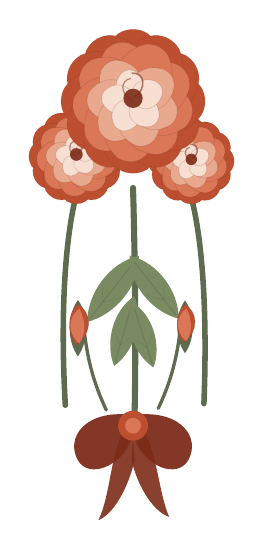
\begin{tikzpicture}
\definecolor{deep}{HTML}{7C2B18}
\definecolor{petal}{HTML}{BC4F30}
\definecolor{mid}{HTML}{D97757}
\definecolor{light}{HTML}{E8A98F}
\definecolor{cream}{HTML}{F7DFD1}
\definecolor{stemc}{HTML}{5E6B4F}
\definecolor{leafc}{HTML}{7A8B62}

% 一朵花：四层花瓣，由外向内变浅
\newcommand{\ring}[3]{% 角度列表, 颜色, 缩放
  \foreach \a in {#1}{%
    \begin{scope}[rotate=\a,scale=#3]
      \fill[#2, draw=deep, line width=0.25pt, draw opacity=0.18]
        (0,0) .. controls (0.46,0.03) and (0.62,0.58) .. (0.19,0.92)
        .. controls (0.07,0.99) and (-0.07,0.99) .. (-0.19,0.92)
        .. controls (-0.62,0.58) and (-0.46,0.03) .. cycle;
    \end{scope}}}

\newcommand{\bloom}[3]{%
  \begin{scope}[shift={(#1,#2)},scale=#3]
    \ring{0,30,60,90,120,150,180,210,240,270,300,330}{petal}{1.0}
    \ring{16,56,96,136,176,216,256,296,336}{mid}{0.84}
    \ring{34,88,142,196,250,304}{light}{0.64}
    \ring{10,82,154,226,298}{cream}{0.44}
    \fill[deep, opacity=0.9] (0,0.04) circle (0.13);
    \draw[deep, line width=0.55pt, opacity=0.6] (0.02,0.06)
      .. controls (0.19,0.16) and (0.16,0.40) .. (-0.02,0.38);
    \draw[deep, line width=0.45pt, opacity=0.5] (-0.02,0.02)
      .. controls (-0.17,0.10) and (-0.18,0.28) .. (-0.03,0.31);
  \end{scope}}

% 花苞：萼片 + 一点花瓣
\newcommand{\bud}[2]{%
  \begin{scope}[shift={(#1)},scale={#2}]
    \fill[stemc] (0,0) .. controls (0.18,0.26) and (0.12,0.62) .. (0,0.78)
      .. controls (-0.12,0.62) and (-0.18,0.26) .. cycle;
    \fill[petal, draw=deep, line width=0.25pt, draw opacity=0.2]
      (-0.02,0.16) .. controls (0.22,0.34) and (0.18,0.62) .. (0,0.72)
      .. controls (-0.16,0.60) and (-0.14,0.28) .. cycle;
    \fill[mid] (0.02,0.18) .. controls (-0.16,0.32) and (-0.13,0.56) .. (0.02,0.66)
      .. controls (0.11,0.50) and (0.11,0.30) .. cycle;
  \end{scope}}

% 叶子：细长 + 中脉
\newcommand{\leaf}[4]{%
  \begin{scope}[shift={(#1,#2)},rotate=#3,scale=#4]
    \fill[leafc] (0,0) .. controls (0.24,0.30) and (0.28,0.84) .. (0,1.18)
      .. controls (-0.28,0.84) and (-0.24,0.30) .. cycle;
    \draw[stemc, line width=0.4pt, opacity=0.45] (0,0.06) -- (0,1.06);
    \draw[stemc, line width=0.3pt, opacity=0.25] (0,0.35) -- (0.16,0.56);
    \draw[stemc, line width=0.3pt, opacity=0.25] (0,0.35) -- (-0.16,0.56);
  \end{scope}}

% 梗
\draw[stemc, line width=2.0pt, line cap=round]
  (-0.86,-2.24) .. controls (-0.92,-1.20) and (-0.88,-0.20) .. (-0.72,0.44);
\draw[stemc, line width=2.2pt, line cap=round]
  (0.02,-2.34) .. controls (0.04,-1.30) and (0.02,-0.20) .. (0.0,0.52);
\draw[stemc, line width=2.0pt, line cap=round]
  (0.90,-2.22) .. controls (0.94,-1.20) and (0.90,-0.22) .. (0.74,0.40);
\draw[stemc, line width=1.2pt, line cap=round]
  (-0.34,-2.30) .. controls (-0.52,-1.92) and (-0.58,-1.62) .. (-0.62,-1.30);
\draw[stemc, line width=1.2pt, line cap=round]
  (0.32,-2.28) .. controls (0.50,-1.90) and (0.56,-1.60) .. (0.60,-1.28);

% 花
\bloom{-0.72}{0.92}{0.62}
\bloom{0.74}{0.86}{0.56}
\bloom{0.0}{1.62}{0.94}

% 叶
\leaf{-0.58}{-1.18}{-38}{0.90}
\leaf{0.58}{-1.14}{38}{0.86}
\leaf{-0.24}{-1.74}{-16}{0.78}
\leaf{0.26}{-1.76}{18}{0.74}

% 花苞
\bud{-0.70,-1.62}{0.92}
\bud{0.66,-1.58}{0.86}

% 缎带：两个环、结、两条飘带
\fill[deep, opacity=0.94] (-0.04,-2.36)
  .. controls (-0.62,-2.30) and (-0.86,-2.66) .. (-0.70,-2.94)
  .. controls (-0.56,-3.18) and (-0.14,-3.02) .. (-0.02,-2.66)
  .. controls (0.02,-2.52) and (-0.01,-2.42) .. (-0.04,-2.36);
\fill[deep, opacity=0.94] (0.04,-2.36)
  .. controls (0.62,-2.30) and (0.86,-2.66) .. (0.70,-2.94)
  .. controls (0.56,-3.18) and (0.14,-3.02) .. (0.02,-2.66)
  .. controls (-0.02,-2.52) and (0.01,-2.42) .. (0.04,-2.36);
\fill[deep, opacity=0.9] (-0.02,-2.40)
  .. controls (-0.30,-2.74) and (-0.26,-3.32) .. (-0.44,-3.70)
  .. controls (-0.24,-3.62) and (-0.06,-3.28) .. (0.02,-2.94) -- cycle;
\fill[deep, opacity=0.9] (0.02,-2.40)
  .. controls (0.32,-2.72) and (0.30,-3.30) .. (0.46,-3.66)
  .. controls (0.24,-3.58) and (0.06,-3.26) .. (-0.02,-2.94) -- cycle;
\fill[petal] (0,-2.50) circle (0.19);
\fill[mid] (0,-2.50) circle (0.10);
\end{tikzpicture}
\end{document}
